%%%%%%%%%%%%%%%%%%%%%%%%%%%%%%%%%%%%%%%%%%%%%%%%%%%%%%%%%%%%%%%%%%%%%%%%%%%%%%%%%%
\begin{frame}[fragile]\frametitle{}

\begin{center}
{\Large Overview}
\end{center}
\end{frame}

%%%%%%%%%%%%%%%%%%%%%%%%%%%%%%%%%%%%%%%%%%%%%%%%%%%%%%%%%%%%%%%%%%%%%%%%%%%%%%%%%%
\begin{frame}[fragile]\frametitle{xkcd}
\begin{center}
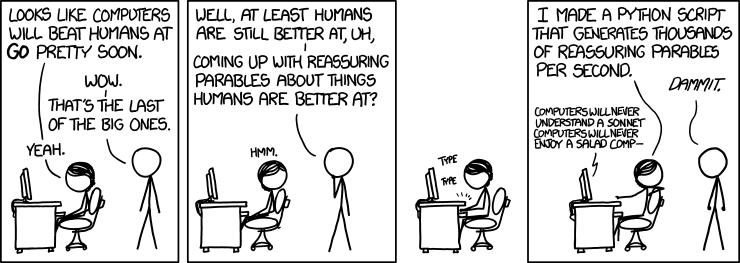
\includegraphics[width=\linewidth,keepaspectratio]{nlpxkcd}
\end{center}

{\tiny (Parables: verse/short stories with morals)}
\end{frame}

%%%%%%%%%%%%%%%%%%%%%%%%%%%%%%%%%%%%%%%%%%%%%%%%%%%%%%%%%%%%%%%%%%%%%%%%%%%%%%%%%%
\begin{frame}[fragile]\frametitle{NLP is AI}
Can Machine understand the way humans do?
\end{frame}

%%%%%%%%%%%%%%%%%%%%%%%%%%%%%%%%%%%%%%%%%%%%%%%%%%%%%%%%%%%%%%%%%%%%%%%%%%%%%%%%%%
\begin{frame}[fragile]\frametitle{Can Machine Answer?}
\begin{center}
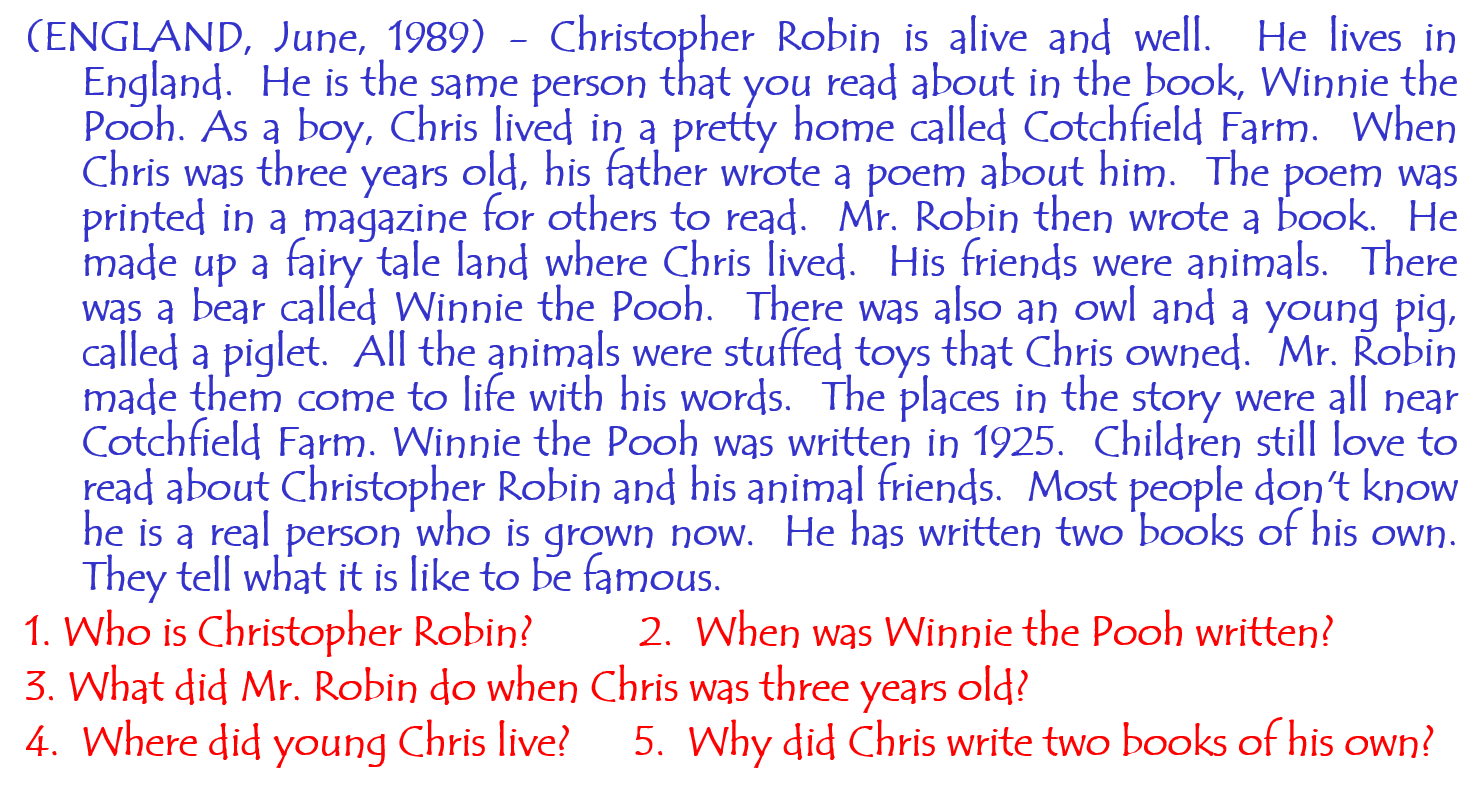
\includegraphics[width=\linewidth,keepaspectratio]{nlproth1}
\end{center}

\tiny{(Ref: CS598 DNR FALL 2005 Machine Learning in Natural Language - Dan Roth
University of Illinois, Urbana-Champaign)}
\end{frame}

%%%%%%%%%%%%%%%%%%%%%%%%%%%%%%%%%%%%%%%%%%%%%%%%%%%%%%%%%%%%%%%%%%%%%%%%%%%%%%%%%%
\begin{frame}[fragile]\frametitle{Understanding Questions}
  \begin{itemize}
    \item What is the question asking? (different from Googling) 
    \item Beyond finding candidate passages; choose the right one.
	\item Say, Q: What is the fastest automobile in the world?
\item A1: \ldots will stretch Volkswagen’s lead in the world’s fastest 
growing vehicle market. Demand for cars is expected to soar \ldots
\item A2: \ldots  the Jaguar XJ220 is the dearest (415,000 pounds), fastest (217mph) and most sought after car in the world.
\item And, what if the answers require aggregation

  \end{itemize}
\end{frame}

%%%%%%%%%%%%%%%%%%%%%%%%%%%%%%%%%%%%%%%%%%%%%%%%%%%%%%%%%%%%%%%%%%%%%%%%%%%%%%%%%%
\begin{frame}[fragile]\frametitle{Not So Easy}
\begin{center}

\includegraphics[width=\linewidth,keepaspectratio]{nlproth2}
\end{center}

Humans may not follow other humans, then what for the machines. But still we can attempt.

Need to study the language well!!!

\tiny{(Ref: CS598 DNR FALL 2005 Machine Learning in Natural Language - Dan Roth
University of Illinois, Urbana-Champaign)}
\end{frame}

%%%%%%%%%%%%%%%%%%%%%%%%%%%%%%%%%%%%%%%%%%%%%%%%%%%%%%%%%%%%%%%%%%%%%%%%%%%%%%%%%%
\begin{frame}[fragile]\frametitle{What's a Language?}
\begin{center}
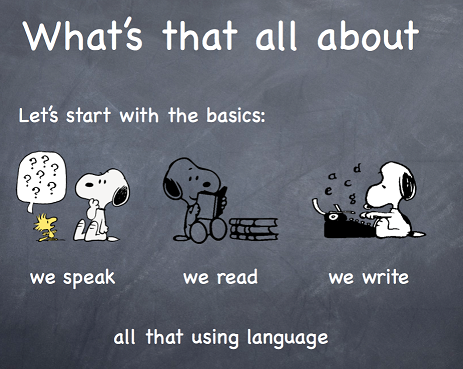
\includegraphics[width=0.8\linewidth,keepaspectratio]{nlp_basics}
\end{center}
\end{frame}

%%%%%%%%%%%%%%%%%%%%%%%%%%%%%%%%%%%%%%%%%%%%%%%%%%%%%%%%%%%%%%%%%%%%%%%%%%%%%%%%%%
\begin{frame}[fragile]\frametitle{What's a Language?}
\begin{center}
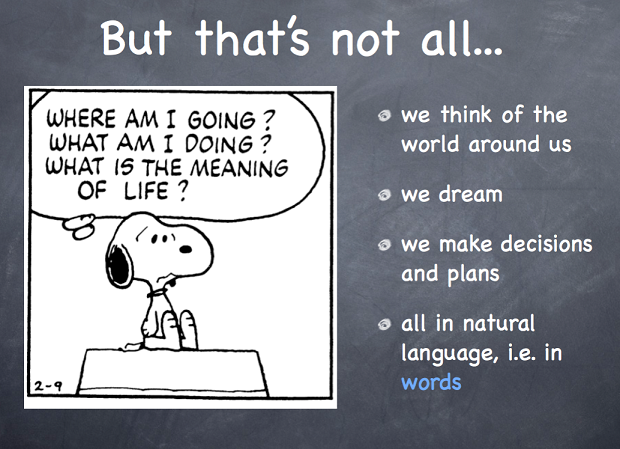
\includegraphics[width=0.8\linewidth,keepaspectratio]{not_all}
\end{center}
\end{frame}



%%%%%%%%%%%%%%%%%%%%%%%%%%%%%%%%%%%%%%%%%%%%%%%%%%%%%%%%%%%%%%%%%%%%%%%%%%%%%%%%%%
\begin{frame}[fragile] \frametitle{$Words == Meaning$?}
 \begin{center}
When you read the word, say, ``Crab'', what does this mean to you?



Bunch of letters? or something else?
\end{center}
\end{frame}

%%%%%%%%%%%%%%%%%%%%%%%%%%%%%%%%%%%%%%%%%%%%%%%%%%%%%%%%%%%%%%%%%%%%%%%%%%%%%%%%%%
\begin{frame}[fragile] \frametitle{$Words == Meaning$?}
\begin{center}

\includegraphics[width=0.8\linewidth,keepaspectratio]{crab1}
\end{center}
Is the symbol representative of its meaning? 
\end{frame}


%%%%%%%%%%%%%%%%%%%%%%%%%%%%%%%%%%%%%%%%%%%%%%%%%%%%%%%%%%%%%%%%%%%%%%%%%%%%%%%%%%
\begin{frame}[fragile] \frametitle{$Words == Meaning$?}
Now, which of these you can understand?

\begin{center}
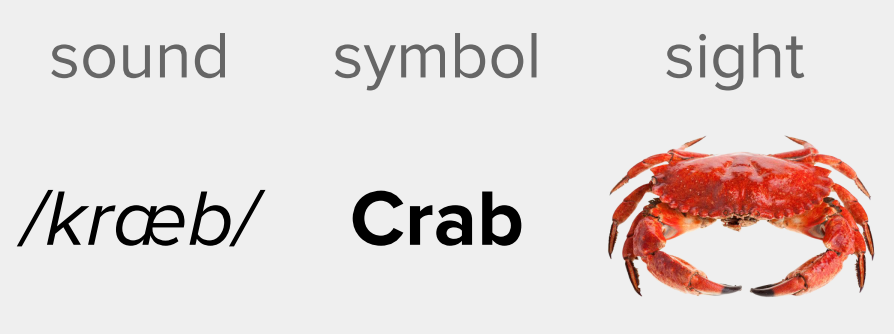
\includegraphics[width=0.8\linewidth,keepaspectratio]{crab2}
\end{center}
Or is it just a mapping in a mental lexicon/vocabulary/dictionary (word, picture, understanding)?
\end{frame}


%%%%%%%%%%%%%%%%%%%%%%%%%%%%%%%%%%%%%%%%%%%%%%%%%%%%%%%%%%%%%%%%%%%%%%%%%%%%%%%%%%
\begin{frame}[fragile]\frametitle{}
\begin{center}
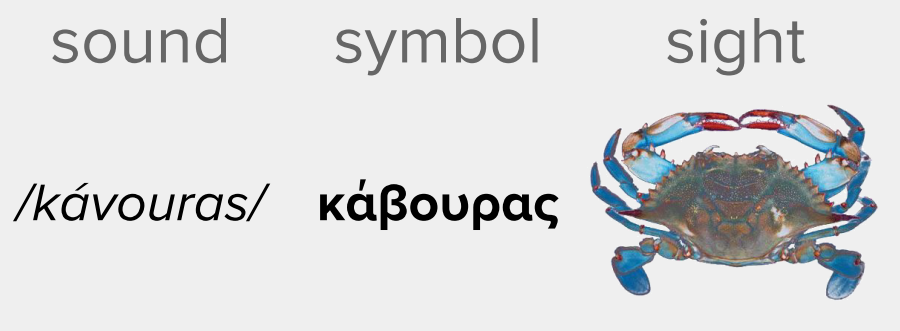
\includegraphics[width=0.8\linewidth,keepaspectratio]{crab3}
\end{center}
These symbols are arbitrary. Do the words, embed knowledge by themselves?

But words is the only thing we have for processing? Then how what can be done?

Verbal and Written communication is primarily though words.
\end{frame}

%%%%%%%%%%%%%%%%%%%%%%%%%%%%%%%%%%%%%%%%%%%%%%%%%%%%%%%%%%%%%%%%%%%%%%%%%%%%%%%%%%
\begin{frame}[fragile] \frametitle{Why should we analyze words?}
Words/Language is:

  \begin{itemize}
    \item Main channel of  Communication
    \item Knowledge Acquisition
  \end{itemize}

  % A grand application: Human computer interaction.
\end{frame}


%%%%%%%%%%%%%%%%%%%%%%%%%%%%%%%%%%%%%%%%%%%%%%%%%%%%%%%%%%%%%%%%%%%%%%%%%%%%%%%%%%
\begin{frame}[fragile] \frametitle{Knowledge and Communication in Language}
  \begin{itemize}
    \item Human knowledge, human communication, is expressed in language
    \item Language technologies: process human language automatically
	\item Examples:
%    \item Two facets of the multilingual information society:
\begin{itemize}
    \item Hand-held devices: predictive text, handwriting recognition
    \item Web search engines: access to information locked up in text
%      \item Natural human-machine interfaces
%      \item Access to stored information
\end{itemize}
  \end{itemize}
\end{frame}

%%%%%%%%%%%%%%%%%%%%%%%%%%%%%%%%%%%%%%%%%%%%%%%%%%%%%%%%%%%%%%%%%%%%%%%%%%%%%%%%%%
\begin{frame}[fragile]\frametitle{Questions}
  \begin{itemize}
    \item   Which Language systems you have recently used?
    \item What is impressive about these systems? (Imagine you stepped out of time machine from the 1970s or 1870s)
    \item How could these systems be improved?
  \end{itemize}
\end{frame}
  


%%%%%%%%%%%%%%%%%%%%%%%%%%%%%%%%%%%%%%%%%%%%%%%%%%%%%%%%%%%%%%%%%%%%%%%%%%%%%%%%%%
\begin{frame}[fragile]\frametitle{Why Language Processing, and why now?}
  \begin{itemize}
    \item  Data: There is huge wealth of human knowledge that has been digitized. A Twitter firehouse of current events and trending topics.
    \item Compute: Our computers are very fast and there are ways to scale out.
    \item Algorithms: Using a combination of CS, ML, linguistic technique we can get the insight quickly.
  \end{itemize}

\end{frame}
 
%%%%%%%%%%%%%%%%%%%%%%%%%%%%%%%%%%%%%%%%%%%%%%%%%%%%%%%%%%%%%%%%%%%%%%%%%%%%%%%%%%
\begin{frame}[fragile]\frametitle{Leveraging Big Data}
  \begin{itemize}
  \item Examples are easier to create than rules.
  \item Rules and logic miss frequency and language dynamics
  \item More data is better for machine learning, relevance is in the long tail
  \item Knowledge engineering is not scalable
  \item Computational linguistics methodologies are stochastic
  \end{itemize}
Question: What do computers like more numbers or words?
\end{frame}



%%%%%%%%%%%%%%%%%%%%%%%%%%%%%%%%%%%%%%%%%%%%%%%%%%%%%%%%%%%%%%%%%%%%%%%%%%%%%%%%%%
\begin{frame}[fragile]\frametitle{Questions}
  \begin{itemize}
    \item How do we write programs to manipulate natural language?
    \item What questions about language could we answer?
    \item How would the programs work?
    \item What data would they need?
    \item First: what do they look like?
  \end{itemize}
\end{frame}

%%%%%%%%%%%%%%%%%%%%%%%%%%%%%%%%%%%%%%%%%%%%%%%%%%%%%%%%%%%%%%%%%%%%%%%%%%%%%%%%%%
\begin{frame}[fragile]\frametitle{}

\begin{center}
{\Large What is Natural Language Processing?}
\end{center}
\end{frame}


%%%%%%%%%%%%%%%%%%%%%%%%%%%%%%%%%%%%%%%%%%%%%%%%%%%%%%%%%%%%%%%%%%%%%%%%%%%%%%%%%%%
%\begin{frame}[fragile]\frametitle{What is Natural Language Processing?}
%\begin{center}
%The science that has been developed around the facts of language 
%passed through three stages before finding its true and unique 
%object. First something called ''grammar'' was studied. This study, 
%initiated by the Greeks and continued mainly by the French, was 
%based on logic. It lacked a scientific approach and was detached 
%from language itself. Its only aim was to give rules for 
%distinguishing between correct and incorrect forms; it was a 
%normative discipline, far removed from actual observation, and its 
%scope was limited.
%
%\end{center}
%-- Ferdinand de Saussure
%\end{frame}

%%%%%%%%%%%%%%%%%%%%%%%%%%%%%%%%%%%%%%%%%%%%%%%%%%%%%%%%%%%%%%%%%%%%%%%%%%%%%%%%%%
\begin{frame}[fragile]\frametitle{What is NLP?}
Natual Language Processing
  \begin{itemize}
\item Natural Language: languages spoken by people (English, French, German, etc.) as opposed to artificial languages, also called as Formal, (C++, Java, Python, etc.) built for computer manipulation
\item Natural Language Processing: computer applications that automatically analyze natural language
  \end{itemize}
\end{frame}


%%%%%%%%%%%%%%%%%%%%%%%%%%%%%%%%%%%%%%%%%%%%%%%%%%%%%%%%%%%%%%%%%%%%%%%%%%%%%%%%%%
\begin{frame}[fragile]\frametitle{What is NLP?}
  \begin{itemize}
    \item  Language = Words + Rules + Exceptions + \ldots
	\item Formally: dictionary (vocabulary) + grammar + \ldots
\item Dictionary : set of words defined in the language (static or dynamic)
\item Grammar: set of rules which describe what is allowable in a language
  \end{itemize}
\end{frame}


%%%%%%%%%%%%%%%%%%%%%%%%%%%%%%%%%%%%%%%%%%%%%%%%%%%
\begin{frame}[fragile] \frametitle{Formal vs. Natural Languages}

\adjustbox{valign=t}{
\begin{minipage}{0.45\linewidth}
Formal Languages
\begin{itemize}
\item Strict, unchanging rules defined by grammars and parsed by regular expressions
\item Generally application specific (chemistry, math)
\item Literal: exactly what is said is meant. 
\item No ambiguity 
\item Parsable by regular expressions
\item Inflexible: no new terms or meaning.
\end{itemize}
\end{minipage}
}
\hfill
\adjustbox{valign=t}{
\begin{minipage}{0.45\linewidth}
Natural Languages
\begin{itemize}
\item Flexible, evolving language that  occurs naturally in human 
communication
\item Unspecific and used in many  domains and applications 
\item  Redundant and verbose in order to make up for ambiguity
\item Expressive 
\item Difficult to parse 
\item Very flexible even in narrow contexts

\end{itemize}
\end{minipage}
}

\end{frame}



%%%%%%%%%%%%%%%%%%%%%%%%%%%%%%%%%%%%%%%%%%%%%%%%%%%%%%%%%%%%%%%%%%%%%%%%%%%%%%%%%%
\begin{frame}[fragile]\frametitle{The Richness of Natual Language}
\begin{itemize}
\item Basic needs and lofty aspirations; technical know-how and
 flights of fantasy
\item Ideas are shared over great separations of distance and time
\end{itemize}

Examples (think of processing these!!!): 
\scriptsize

\begin{itemize}
\item Overhead the day drives level and grey, hiding the sun by a flight
  of grey spears.  (William Faulkner, \textit{As I Lay Dying}, 1935)
\item When using the toaster please ensure that the exhaust fan is turned
  on. (sign in dormitory kitchen)
\item Amiodarone weakly inhibited CYP2C9, CYP2D6, and CYP3A4-mediated
  activities with Ki values of 45.1-271.6 $\mu$M (Medline)
\item Iraqi Head Seeks Arms (spoof headline, \url{http://www.snopes.com/humor/nonsense/head97.htm}
\item The earnest prayer of a righteous man has great power and wonderful
  results. (James 5:16b)
\item Twas brillig, and the slithy toves did gyre and gimble in the wabe
  (Lewis Carroll, \textit{Jabberwocky}, 1872)
\item There are two ways to do this, AFAIK :smile:  (internet discussion archive)
\end{itemize}
\end{frame}

%%%%%%%%%%%%%%%%%%%%%%%%%%%%%%%%%%%%%%%%%%%%%%%%%%%%%%%%%%%%%%%%%%%%%%%%%%%%%%%%%%
\begin{frame}[fragile]\frametitle{}

\begin{center}
{\Large History of NLP/Text/Linguistics, a western view}
\end{center}
\end{frame}

  
%%%%%%%%%%%%%%%%%%%%%%%%%%%%%%%%%%%%%%%%%%%%%%%%%%%%%%%%%%%%%%%%%%%%%%%%%%%%%%%%%%
\begin{frame}[fragile]\frametitle{History of NLP}
\begin{center}
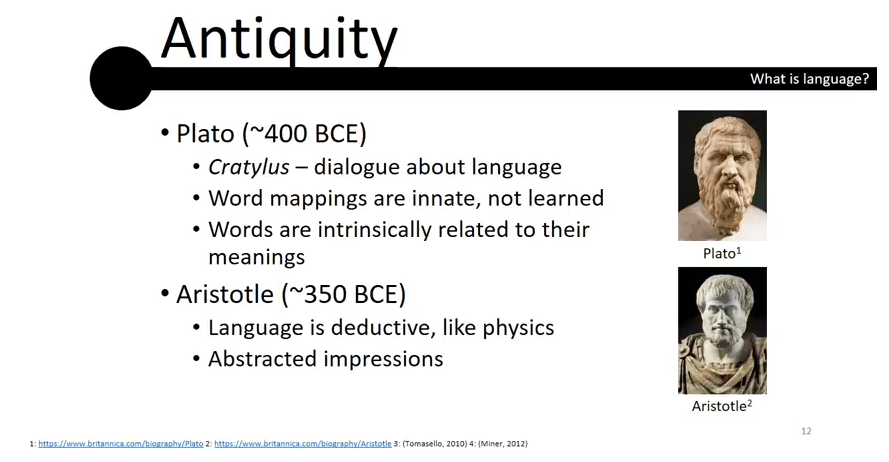
\includegraphics[width=\linewidth,keepaspectratio]{nlphist1}
\end{center}

{\tiny Note: A deductive language is a computer programming language in which the program is a collection of predicates ('facts') and rules that connect them. Such a language is used to create knowledge based systems or expert systems which can deduce answers to problem sets by applying the rules to the facts they have been given.

(Ref: Text Mining - Jeff Shaul)}
\end{frame}

%%%%%%%%%%%%%%%%%%%%%%%%%%%%%%%%%%%%%%%%%%%%%%%%%%%%%%%%%%%%%%%%%%%%%%%%%%%%%%%%%%
\begin{frame}[fragile]\frametitle{History of NLP}
\begin{center}
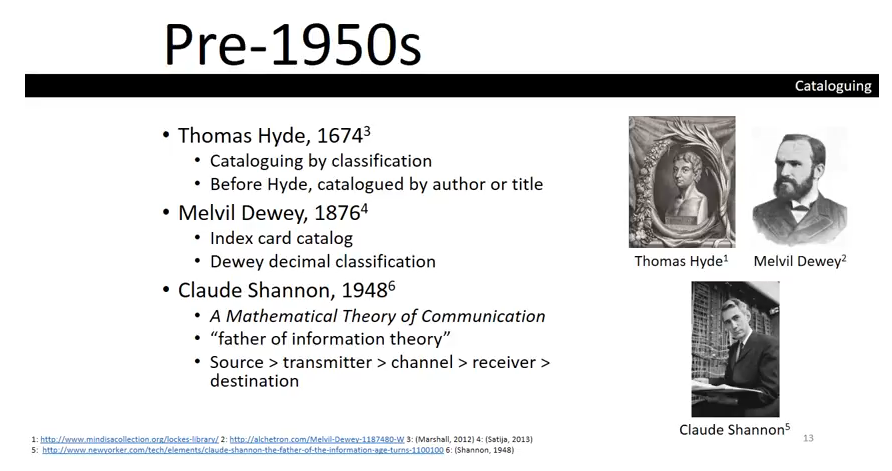
\includegraphics[width=\linewidth,keepaspectratio]{nlphist2}
\end{center}

{\tiny (Ref: Text Mining - Jeff Shaul)}
\end{frame}


%%%%%%%%%%%%%%%%%%%%%%%%%%%%%%%%%%%%%%%%%%%%%%%%%%%%%%%%%%%%%%%%%%%%%%%%%%%%%%%%%%
\begin{frame}[fragile]\frametitle{History of NLP}
\begin{center}
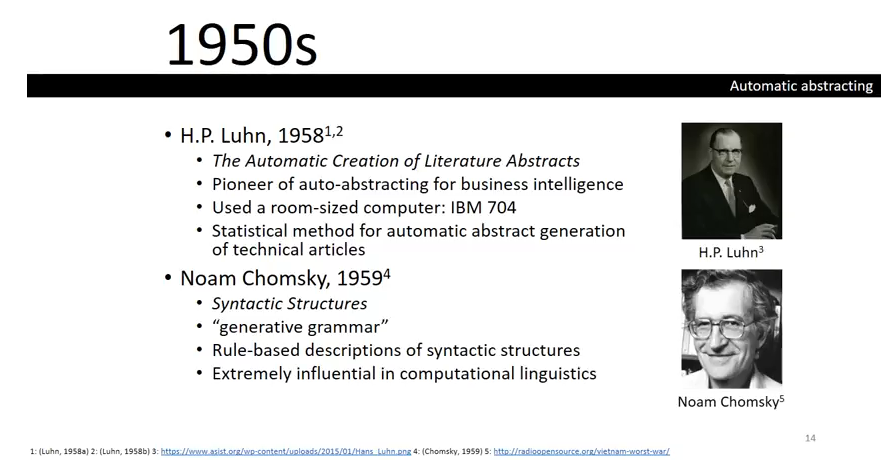
\includegraphics[width=\linewidth,keepaspectratio]{nlphist3}
\end{center}

{\tiny (Ref: Text Mining - Jeff Shaul)}
\end{frame}


%%%%%%%%%%%%%%%%%%%%%%%%%%%%%%%%%%%%%%%%%%%%%%%%%%%%%%%%%%%%%%%%%%%%%%%%%%%%%%%%%%
\begin{frame}[fragile]\frametitle{History of NLP}
\begin{center}
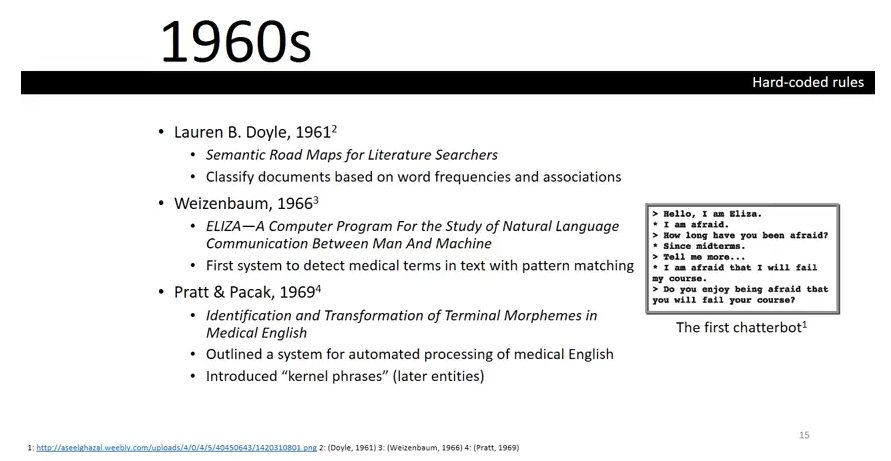
\includegraphics[width=\linewidth,keepaspectratio]{nlphist4}
\end{center}

{\tiny (Ref: Text Mining - Jeff Shaul)}
\end{frame}


%%%%%%%%%%%%%%%%%%%%%%%%%%%%%%%%%%%%%%%%%%%%%%%%%%%%%%%%%%%%%%%%%%%%%%%%%%%%%%%%%%
\begin{frame}[fragile]\frametitle{History of NLP}
\begin{center}
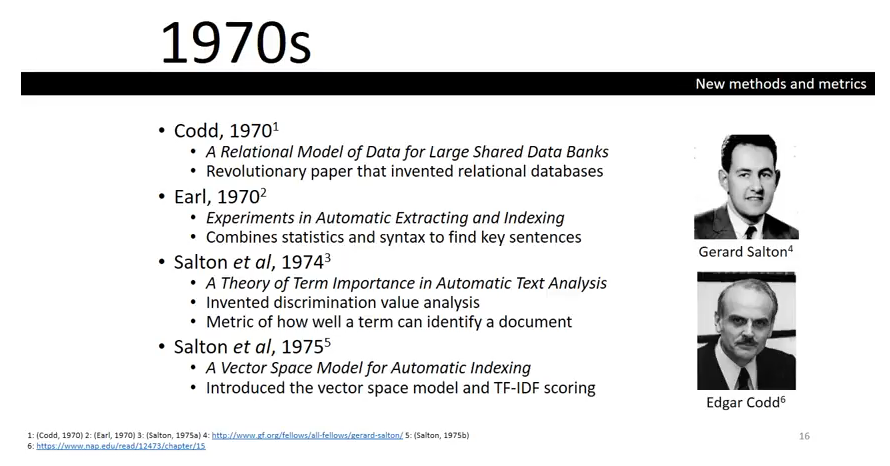
\includegraphics[width=\linewidth,keepaspectratio]{nlphist5}
\end{center}

{\tiny (Ref: Text Mining - Jeff Shaul)}
\end{frame}


%%%%%%%%%%%%%%%%%%%%%%%%%%%%%%%%%%%%%%%%%%%%%%%%%%%%%%%%%%%%%%%%%%%%%%%%%%%%%%%%%%
\begin{frame}[fragile]\frametitle{History of NLP}
\begin{center}
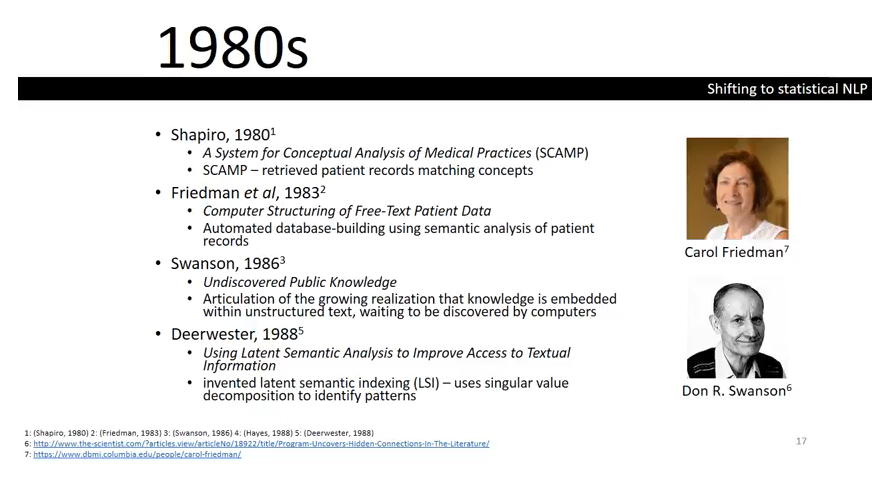
\includegraphics[width=\linewidth,keepaspectratio]{nlphist6}
\end{center}

{\tiny (Ref: Text Mining - Jeff Shaul)}
\end{frame}


%%%%%%%%%%%%%%%%%%%%%%%%%%%%%%%%%%%%%%%%%%%%%%%%%%%%%%%%%%%%%%%%%%%%%%%%%%%%%%%%%%
\begin{frame}[fragile]\frametitle{History of NLP}
\begin{center}
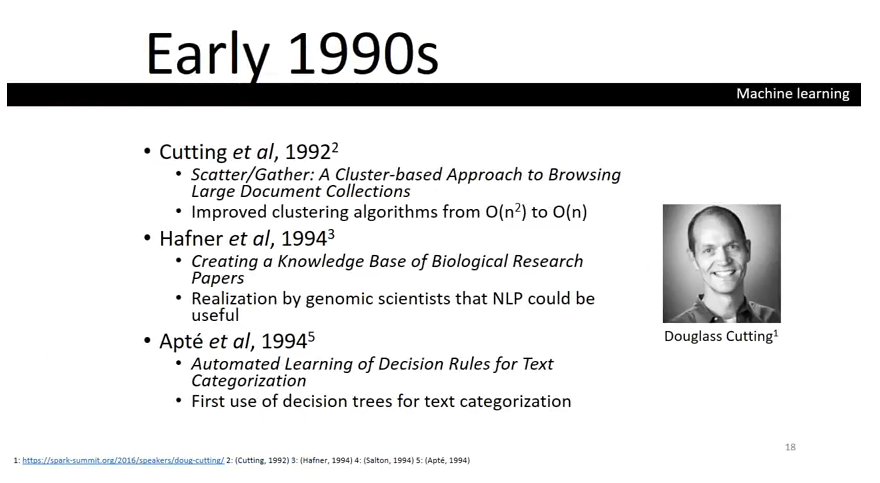
\includegraphics[width=\linewidth,keepaspectratio]{nlphist7}
\end{center}

{\tiny (Ref: Text Mining - Jeff Shaul)}
\end{frame}


%%%%%%%%%%%%%%%%%%%%%%%%%%%%%%%%%%%%%%%%%%%%%%%%%%%%%%%%%%%%%%%%%%%%%%%%%%%%%%%%%%
\begin{frame}[fragile]\frametitle{History of NLP}
\begin{center}
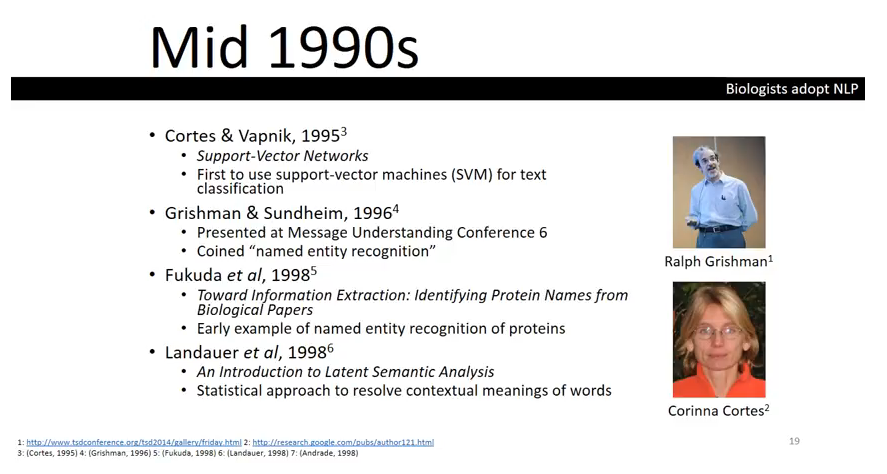
\includegraphics[width=\linewidth,keepaspectratio]{nlphist8}
\end{center}

{\tiny (Ref: Text Mining - Jeff Shaul)}
\end{frame}


%%%%%%%%%%%%%%%%%%%%%%%%%%%%%%%%%%%%%%%%%%%%%%%%%%%%%%%%%%%%%%%%%%%%%%%%%%%%%%%%%%
\begin{frame}[fragile]\frametitle{History of NLP}
\begin{center}
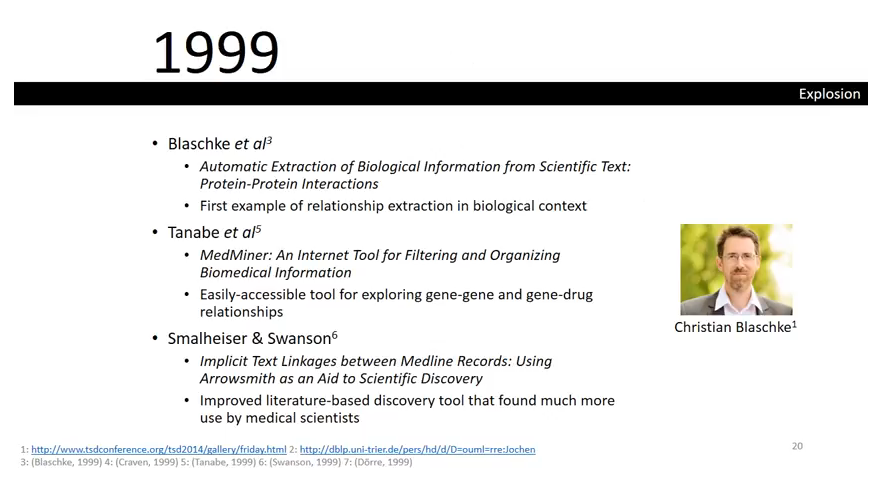
\includegraphics[width=\linewidth,keepaspectratio]{nlphist9}
\end{center}

{\tiny (Ref: Text Mining - Jeff Shaul)}
\end{frame}


%%%%%%%%%%%%%%%%%%%%%%%%%%%%%%%%%%%%%%%%%%%%%%%%%%%%%%%%%%%%%%%%%%%%%%%%%%%%%%%%%%
\begin{frame}[fragile]\frametitle{History of NLP}
\begin{center}
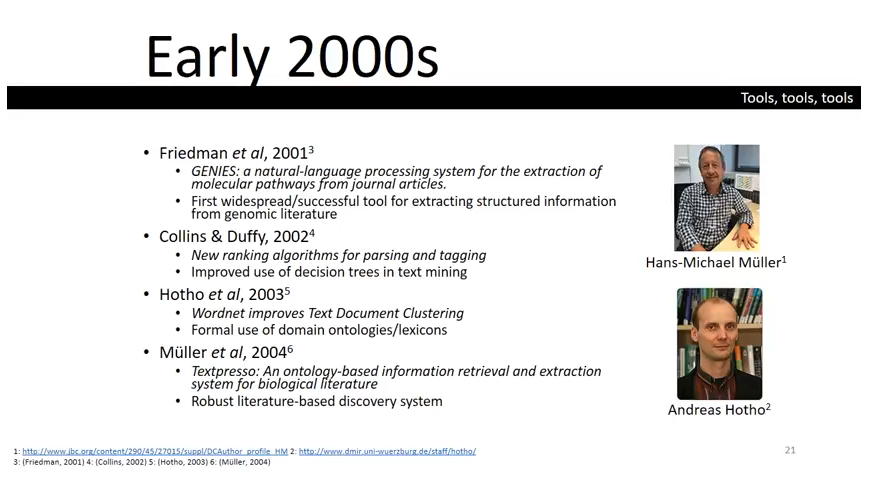
\includegraphics[width=\linewidth,keepaspectratio]{nlphist10}
\end{center}

{\tiny (Ref: Text Mining - Jeff Shaul)}
\end{frame}


%%%%%%%%%%%%%%%%%%%%%%%%%%%%%%%%%%%%%%%%%%%%%%%%%%%%%%%%%%%%%%%%%%%%%%%%%%%%%%%%%%
\begin{frame}[fragile]\frametitle{History of NLP}
\begin{center}
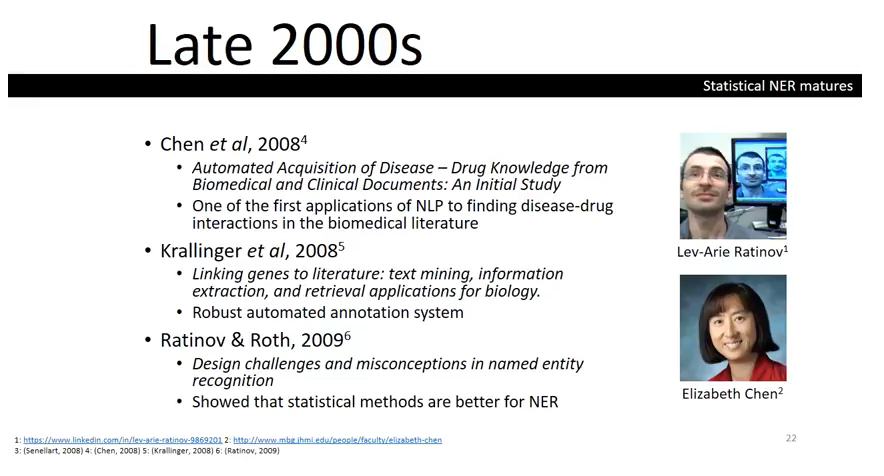
\includegraphics[width=\linewidth,keepaspectratio]{nlphist11}
\end{center}

{\tiny (Ref: Text Mining - Jeff Shaul)}
\end{frame}


%%%%%%%%%%%%%%%%%%%%%%%%%%%%%%%%%%%%%%%%%%%%%%%%%%%%%%%%%%%%%%%%%%%%%%%%%%%%%%%%%%
\begin{frame}[fragile]\frametitle{History of NLP}
\begin{center}
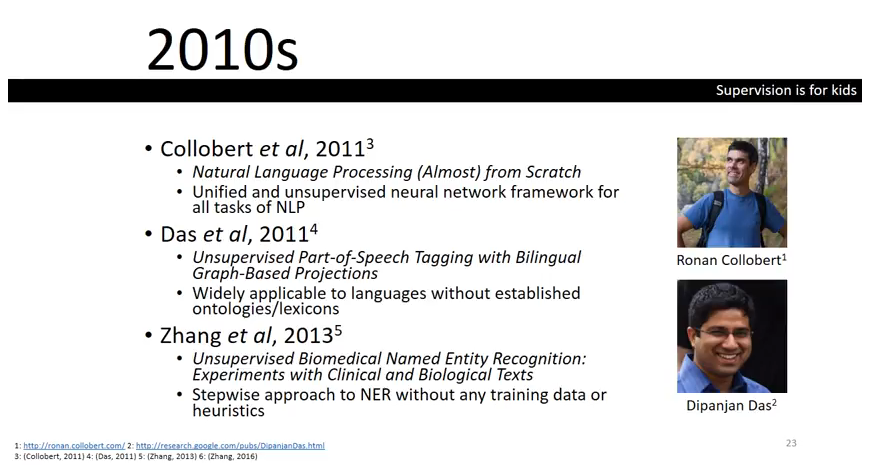
\includegraphics[width=\linewidth,keepaspectratio]{nlphist12}
\end{center}

{\tiny (Ref: Text Mining - Jeff Shaul)}
\end{frame}


%%%%%%%%%%%%%%%%%%%%%%%%%%%%%%%%%%%%%%%%%%%%%%%%%%%%%%%%%%%%%%%%%%%%%%%%%%%%%%%%%%
\begin{frame}[fragile]\frametitle{}

\begin{center}
{\Large Why NLP is hard?}
\end{center}
\end{frame}

  
%%%%%%%%%%%%%%%%%%%%%%%%%%%%%%%%%%%%%%%%%%%%%%%%%%%%%%%%%%%%%%%%%%%%%%%%%%%%%%%%%%
\begin{frame}[fragile]\frametitle{Why that is hard?}
NLP itself is hard. Why?
\begin{center}
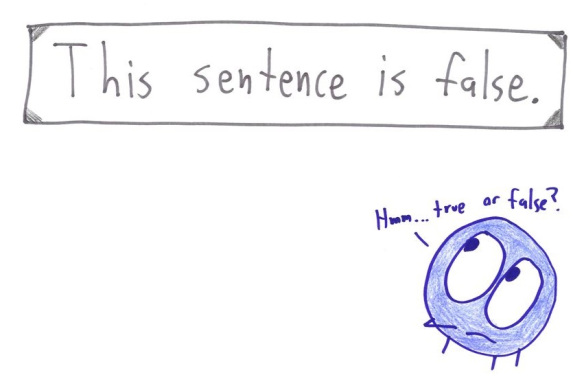
\includegraphics[width=0.6\linewidth,keepaspectratio]{nlphard}
\end{center}
Brainstorm the reasons NLP is hard.
\end{frame}


%%%%%%%%%%%%%%%%%%%%%%%%%%%%%%%%%%%%%%%%%%%%%%%%%%%%%%%%%%%%%%%%%%%%%%%%%%%%%%%%%%
\begin{frame}[fragile]\frametitle{Textual Queries, can NLP answer?}
\begin{exampleblock}{Example 1}
  \begin{description}
    \item [Text] Never before had ski racing, a sport dominated by
      monosyllabic mountain men, seen the likes of Alberto Tomba, the
      flamboyant Bolognese flatlander who at 21 captured two gold
      medals at the Calgary Olympics.
    \item [Hypothesis] Alberto Tomba won a race.
  \end{description}
\end{exampleblock}
\end{frame}

%%%%%%%%%%%%%%%%%%%%%%%%%%%%%%%%%%%%%%%%%%%%%%%%%%%%%%%%%%%%%%%%%%%%%%%%%%%%%%%%%%
\begin{frame}[fragile]\frametitle{Textual Queries, can NLP answer?}
\begin{exampleblock}{Example 2}
  \begin{description}
    \item [Text] Researchers at the Harvard School of Public Health
      say that people who drink coffee may be doing a lot more than
      keeping themselves awake---this kind of consumption apparently
      also can help reduce the risk of diseases.
    \item [Hypothesis] Coffee drinking has health benefits.
  \end{description}
\end{exampleblock}
\end{frame}

%%%%%%%%%%%%%%%%%%%%%%%%%%%%%%%%%%%%%%%%%%%%%%%%%%%%%%%%%%%%%%%%%%%%%%%%%%%%%%%%%%
\begin{frame}[fragile]\frametitle{Why NLP is hard?}
  \begin{itemize}
    \item  Ambiguity: There are many different ways to represent the same thing.
% \item Humans don't consciously understand language. 
\item Language is inherently very high dimensional and sparse. There are a lot of rare words.
\item Out of sample generalization: New words and new sentences all the time.
\item Order and context are extremely important. ''Dog bites man'' and ''Man bites dog'' have vastly different meanings even though they differ by a very small amount.
\item Anything else?
  \end{itemize}

\end{frame}
 
 
%%%%%%%%%%%%%%%%%%%%%%%%%%%%%%%%%%%%%%%%%%%%%%%%%%%%%%%%%%%%%%%%%%%%%%%%%%%%%%%%%%
\begin{frame}[fragile]\frametitle{}

\begin{center}
{\Large Where NLP stands?}
\end{center}
\end{frame}



%%%%%%%%%%%%%%%%%%%%%%%%%%%%%%%%%%%%%%%%%%%%%%%%%%%%%%%%%%%%%%%%%%%%%%%%%%%%%%%%%%
\begin{frame}[fragile]\frametitle{Where is it useful?}
  \begin{itemize}
    \item Information Extraction
    \item Spoken Dialog
    \item Question Answering
    \item Text Summarization
	\item Etc \ldots
  \end{itemize}
\end{frame}

%%%%%%%%%%%%%%%%%%%%%%%%%%%%%%%%%%%%%%%%%%%%%%%%%%%%%%%%%%%%%%%%%%%%%%%%%%%%%%%%%%
\begin{frame}[fragile]\frametitle{Where NLP stands?}
\begin{center}
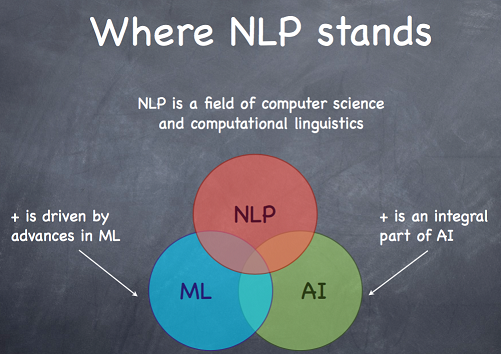
\includegraphics[width=0.8\linewidth,keepaspectratio]{nlpstands}
\end{center}
\end{frame}


%%%%%%%%%%%%%%%%%%%%%%%%%%%%%%%%%%%%%%%%%%%%%%%%%%%%%%%%%%%%%%%%%%%%%%%%%%%%%%%%%%
\begin{frame}[fragile]\frametitle{Main approaches in NLP}
  \begin{itemize}
    \item Rule-based methods: eg Regular expressions.
    \item  Machine learning: eg Linear classifiers.
    \item Deep Learning: eg Recurrent Neural Networks
  \end{itemize}
\end{frame}



%%%%%%%%%%%%%%%%%%%%%%%%%%%%%%%%%%%%%%%%%%%%%%%%%%%%%%%%%%%%%%%%%%%%%%%%%%%%%%%%%%
\begin{frame}[fragile]\frametitle{Example: rule based approach}
Let's say, you want to find slots (City, date, etc) from following sentence:

``Show me flights from Boston to San Francisco on Tuesday''

Context-free grammar is defined by ``rules'' with substitution syntax such as:

  \begin{itemize}
    \item SHOW:   show me | i want | can i see
    \item FLIGHTS:   (a) flight | flights
    \item ORIGIN:   from CITY
    \item DESTINATION: to CITY
    \item CITY:  Boston | San Francisco | Denver | Washington
  \end{itemize}
Need to parse the sentence and wherever you find any of the right-hand side words, you put left hand side annotation

{\tiny (Ref: https://web.stanford.edu/~jurafsky/slp3/29.pdf)}
\end{frame}


%%%%%%%%%%%%%%%%%%%%%%%%%%%%%%%%%%%%%%%%%%%%%%%%%%%%%%%%%%%%%%%%%%%%%%%%%%%%%%%%%%
\begin{frame}[fragile]\frametitle{Explanation: What is Context Free Grammar?}
Context-free grammars are named as such because any of the production rules in the grammar can be applied regardless of context. It does not depend on any other symbols that may or may not be around a given symbol that is having a rule applied to it.

  \begin{itemize}
    \item Context-free Grammars allow a non-terminal to be replaced by a corresponding production rule whenever it appears in a derivation process. The replacement occurs irrespective of what lies before or after the non-terminal. This happens because the LHS of a production rule allows only a single non-terminal of the form :
 
$V \rightarrow (V + T)*$, where $V$ is a non-terminal and $T$ is a terminal

Hence, the dependence on context is removed owing to this restriction.

    \item Context-sensitive Grammars being stronger of the two allows replacement of a non-terminal only based on it’s left or right context,i.e, depending on the terminals or non-terminals that precedes or succeeds it.
  \end{itemize}

{\tiny  (Ref: https://www.quora.com/What-is-the-meaning-of-context-free-in-context-free-grammar )}
\end{frame}



%%%%%%%%%%%%%%%%%%%%%%%%%%%%%%%%%%%%%%%%%%%%%%%%%%%%%%%%%%%%%%%%%%%%%%%%%%%%%%%%%%
\begin{frame}[fragile]\frametitle{Example: rule based approach}

``Show me fligths from Boston to San Francisco on Tuesday''

Parsing results in:

\begin{center}
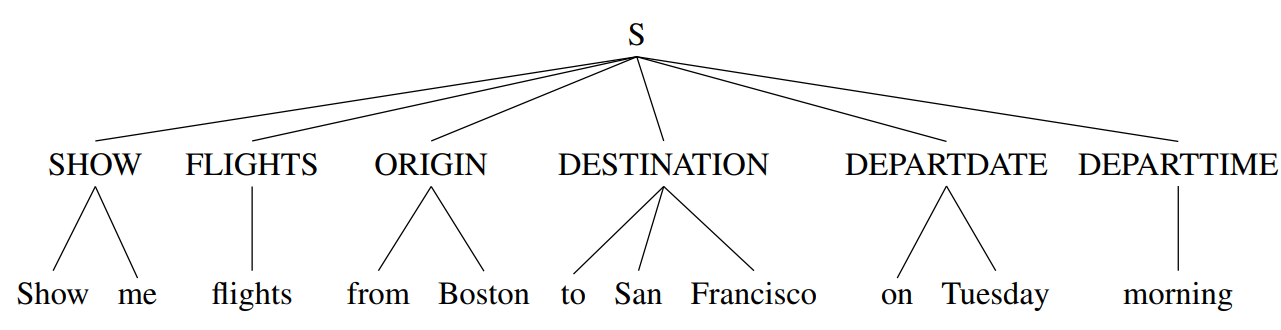
\includegraphics[width=\linewidth,keepaspectratio]{sentcfg}
\end{center}

{\tiny (Ref: https://web.stanford.edu/~jurafsky/slp3/29.pdf)}
\end{frame}

%%%%%%%%%%%%%%%%%%%%%%%%%%%%%%%%%%%%%%%%%%%%%%%%%%%%%%%%%%%%%%%%%%%%%%%%%%%%%%%%%%
\begin{frame}[fragile]\frametitle{Example: machine learning approach}

CRF (Conditional Random Field): probabilistic Named entity recognition.

Training Corpus:

\begin{center}
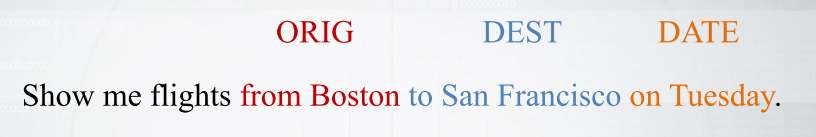
\includegraphics[width=\linewidth,keepaspectratio]{sentner}
\end{center}

Feature engineering:
  \begin{itemize}
    \item  Is the word capitalized?
    \item Is the word in a list of city names?
    \item What is the previous word?
    \item What is the previous slot?
  \end{itemize}

{\tiny (Ref: https://www.coursera.org/learn/language-processing/lecture/j8kee/main-approaches-in-nlp)}
\end{frame}

%%%%%%%%%%%%%%%%%%%%%%%%%%%%%%%%%%%%%%%%%%%%%%%%%%%%%%%%%%%%%%%%%%%%%%%%%%%%%%%%%%
\begin{frame}[fragile]\frametitle{Example: deep learning approach}

LSTM (Long Short Term Memory):
  \begin{itemize}
    \item  Big training corpus
    \item No feature generation
    \item Defining the model
    \item Training and inference
  \end{itemize}


\begin{center}
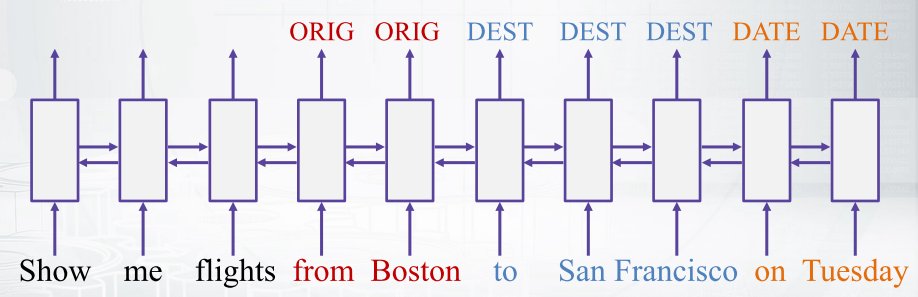
\includegraphics[width=\linewidth,keepaspectratio]{sentlstm}
\end{center}

{\tiny (Ref: https://www.coursera.org/learn/language-processing/lecture/j8kee/main-approaches-in-nlp)}
\end{frame}



%%%%%%%%%%%%%%%%%%%%%%%%%%%%%%%%%%%%%%%%%%%%%%%%%%%%%%%%%%%%%%%%%%%%%%%%%%%%%%%%%%
\begin{frame}[fragile]\frametitle{Goal of NLP}
  \begin{itemize}
    \item  To convert letters, words, and ideas into numbers.
    \item Once we have the numbers we use math and machine learning.
  \end{itemize}
\begin{center}
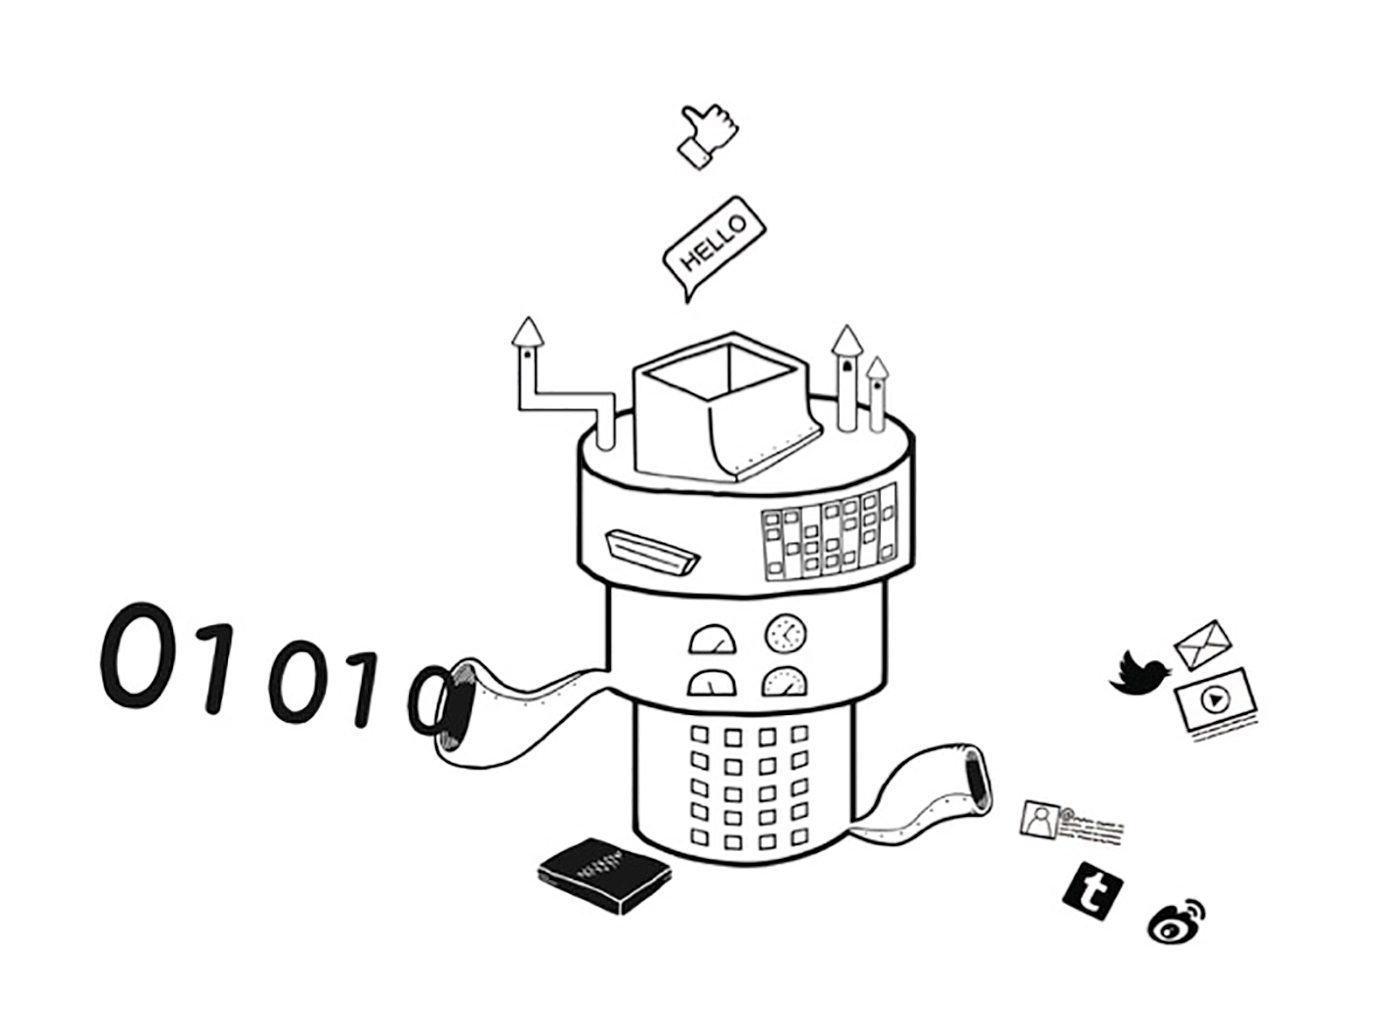
\includegraphics[width=0.6\linewidth,keepaspectratio]{nlpgoal}
\end{center}
\end{frame}


%%%%%%%%%%%%%%%%%%%%%%%%%%%%%%%%%%%%%%%%%%%%%%%%%%%%%%%%%%%%%%%%%%%%%%%%%%%%%%%%%%%
%\begin{frame}[fragile]\frametitle{Textual Inference}
%\begin{exampleblock}{Example 3}
%  \begin{description}
%  \item [Text] Never before had ski racing, a sport dominated by
%    monosyllabic mountain men, seen the likes of Alberto Tomba, the
%    flamboyant Bolognese flatlander who at 21 \textbf{almost} captured
%    two gold medals at the Calgary Olympics.
%    \item [Hypothesis] Alberto Tomba won a race.
%  \end{description}
%\end{exampleblock}
%\end{frame}

%%%%%%%%%%%%%%%%%%%%%%%%%%%%%%%%%%%%%%%%%%%%%%%%%%%%%%%%%%%%%%%%%%%%%%%%%%%%%%%%%%%
%\begin{frame}[fragile]\frametitle{Some Component Technologies}
%  \begin{itemize}
%    \item Word overlap
%    \item Structural correspondence (sentence level parsing)
%    \item Semantic / pragmatic inference 
%    \item Paraphrase at word and phrase level
%    \item Background knowledge
%  \end{itemize}
%\end{frame}
%
%%%%%%%%%%%%%%%%%%%%%%%%%%%%%%%%%%%%%%%%%%%%%%%%%%%%%%%%%%%%%%%%%%%%%%%%%%%%%%%%%%%
%\begin{frame}[fragile]\frametitle{Prospects}
%Still lots of challenges, but
%  \begin{itemize}
%    \item wide-coverage syntactic parsers edging into commodity status;
%    \item NLP is moving out of the lab.
%  \end{itemize}
%\end{frame}

% %%%%%%%%%%%%%%%%%%%%%%%%%%%%%%%%%%%%%%%%%%%%%%%%%%%%%%%%%%%%%%%%%%%%%%%%%%%%%%%%%%
% \begin{frame}[fragile]\frametitle{Domains within NLP}

% \begin{block}{Major sub-domains of NLP}
  % \begin{itemize}
    % \item Understanding
    % \item Translation
    % \item Generation
  % \end{itemize}
% \end{block}

% \begin{block}{Modalities}
  % \begin{itemize}
    % \item Text
    % \item Speech
    % \item Images
  % \end{itemize}
% \end{block}

% \end{frame}

% %%%%%%%%%%%%%%%%%%%%%%%%%%%%%%%%%%%%%%%%%%%%%%%%%%%%%%%%%%%%%%%%%%%%%%%%%%%%%%%%%%%
% %\begin{frame}[fragile]\frametitle{Disciplines Studying Language}
% %\begin{itemize}
% %\item Linguistics
% %\item Translation
% %\item Literary criticism
% %\item Philosophy
% %\item Anthropology
% %\item Psychology
% %\item Law
% %\item Forensics
% %\item Cryptanalysis
% %\end{itemize}
% %\end{frame}

% %%%%%%%%%%%%%%%%%%%%%%%%%%%%%%%%%%%%%%%%%%%%%%%%%%%%%%%%%%%%%%%%%%%%%%%%%%%%%%%%%%
% \begin{frame}[fragile]\frametitle{Language}
% \begin{itemize}
% \item Unprecedented volume of information:  \emph{mostly unstructured.}
% \item 8 Tb books in 2003
% \item 24 hours of scientific literature would take 5 years to read
% \item Fraction of work/leisure time spent navigating this information
% \item A great challenge for natural language processing
% \end{itemize}
% \end{frame}

% %%%%%%%%%%%%%%%%%%%%%%%%%%%%%%%%%%%%%%%%%%%%%%%%%%%%%%%%%%%%%%%%%%%%%%%%%%%%%%%%%%
% \begin{frame}[fragile]\frametitle{Language and the Internet}
% \begin{itemize}
% \item Despite success of web search engines, we need skill, knowledge, and luck to answer the following questions:
  % \begin{itemize}
  % \item \textit{What tourist sites can I visit between Philadelphia and Pittsburgh on a
    % limited budget?}
  % \item \textit{What do expert critics say about Canon digital cameras?}
  % \item \textit{What predictions about the steel market were made by
      % credible commentators in the past week?}
  % \end{itemize}
% \item Requires a combination of language processing tasks, e.g.  information extraction, inference, and summarisation
% \end{itemize}
% \end{frame}


%%%%%%%%%%%%%%%%%%%%%%%%%%%%%%%%%%%%%%%%%%%%%%%%%%%%%%%%%%%%%%%%%%%%%%%%%%%%%%%%%%
\begin{frame}[fragile]\frametitle{The Promise of NLP}
\begin{itemize}
\item Importance in scientific, economic, social and cultural arenas
\item Growing rapidly as its theories and methods are deployed in new technologies
\item Therefore a wide range of people should have a working knowledge of NLP
  \begin{itemize}
  \item Academia: humanities computing, corpus linguistics, computer science, artificial intelligence
  \item Industry: HCI, business information analysis, web software development
  \end{itemize}
\item The goal is to open the field of NLP to a broad audience.
\end{itemize}
\end{frame}

%%%%%%%%%%%%%%%%%%%%%%%%%%%%%%%%%%%%%%%%%%%%%%%%%%%%%%%%%%%%%%%%%%%%%%%%%%%%%%%%%%
\begin{frame}[fragile]\frametitle{NLP and Intelligence}
\begin{itemize}
\item Long-standing challenge to build intelligent machines
\item Chief measure of machine intelligence has been linguistic: Turing test
\end{itemize}
\end{frame}

%%%%%%%%%%%%%%%%%%%%%%%%%%%%%%%%%%%%%%%%%%%%%%%%%%%%%%%%%%%%%%%%%%%%%%%%%%%%%%%%%%
\begin{frame}[fragile]\frametitle{NLP and Intelligence}
\begin{itemize}
\item Research on spoken dialog systems, also MT \emph{--- integrated NLP systems which future users would regard as highly intelligent}
\item Example human-machine dialog:
\small
\begin{tabular}{ll}
S: & How may I help you?\\
U: & When is Saving Private Ryan playing?\\
S: & For what theater?\\
U: & The Paramount theater.\\
S: & Saving Private Ryan is not playing at the Paramount theater,\\
   & but it's playing at the Madison theater at 3:00, 5:30, and 10:30. 
\end{tabular}
\end{itemize}
\end{frame}


%%%%%%%%%%%%%%%%%%%%%%%%%%%%%%%%%%%%%%%%%%%%%%%%%%%%%%%%%%%%%%%%%%%%%%%%%%%%%%%%%%
\begin{frame}[fragile]\frametitle{NLP and Intelligence (cont)}
\begin{itemize}
\item Today's systems limited to narrowly defined domains
\item Couldn't ask above system for other information, e.g.:
  \begin{itemize}
  \item Driving instructions
  \item Details of nearby restaurants
  \end{itemize}
\item To add such support we would have to:
  \begin{itemize}
  \item Store the required information
  \item Incorporate suitable questions and answers into the system
  \end{itemize}
\item Common-sense reasoning vs business logic
\item Need to make progress on natural linguistic interaction without recourse to this unrestricted knowledge and reasoning capability
\end{itemize}
\end{frame}


%
%%%%%%%%%%%%%%%%%%%%%%%%%%%%%%%%%%%%%%%%%%%%%%%%%%%%%%%%%%%%%%%%%%%%%%%%%%%%%%%%%%%
%\begin{frame}[fragile]\frametitle{Language and Symbol Processing}
%\begin{itemize}
%\item Origin of the idea that natural language could be treated computationally: philosophy of language work in early 1900s, to reconstruct mathematical reasoning using logic
%\item Language as a formal system
%%\item Three further developments:
%%  \begin{itemize}
%%  \item Formal language theory
%%  \item Symbolic logic
%%  \item Principle of compositionality
%%  \end{itemize}
%\item More recent developments:
%  \begin{itemize}
%  \item Data-intensive NLP
%  \item Machine learning in NLP
%  \item Evaluation-led methodologies
%  \end{itemize}
%%\item Many interesting philosophical issues (see book)
%%\item Key: balancing act between symbolic and statistical approaches
%\end{itemize}
%\end{frame}

%
%%%%%%%%%%%%%%%%%%%%%%%%%%%%%%%%%%%%%%%%%%%%%%%%%%%%%%%%%%%%%%%%%%%%%%%%%%%%%%%%%%%
%\begin{frame}[fragile]\frametitle{Processing}
%\begin{center}
%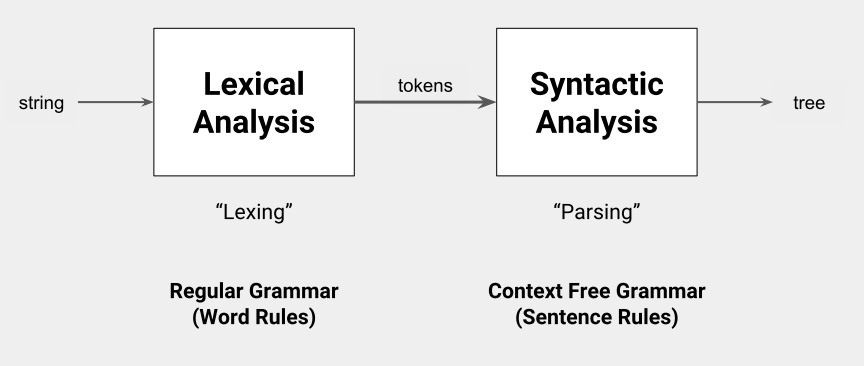
\includegraphics[width=0.8\linewidth,keepaspectratio]{lexproc}
%\end{center}
%Who has written a compiler or interpreter?
%\end{frame}

% %%%%%%%%%%%%%%%%%%%%%%%%%%%%%%%%%%%%%%%%%%%%%%%%%%%%%%%%%%%%%%%%%%%%%%%%%%%%%%%%%%
% \begin{frame}[fragile]\frametitle{The NLP Pipeline}
% \begin{center}
% 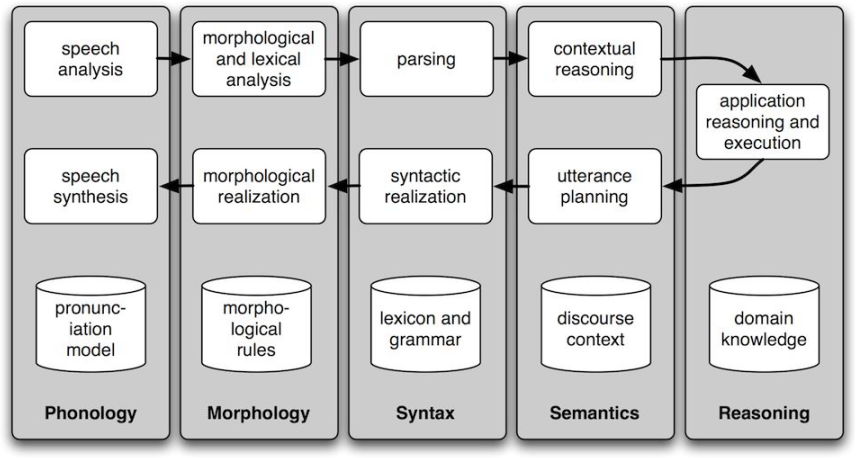
\includegraphics[width=\linewidth,keepaspectratio]{pipe}
% \end{center}
% \end{frame}

%%%%%%%%%%%%%%%%%%%%%%%%%%%%%%%%%%%%%%%%%%%%%%%%%%%%%%%%%%%%%%%%%%%%%%%%%%%%%%%%%%%
%\begin{frame}[fragile]\frametitle{The State of the Art}
%  \begin{itemize}
%  \item Academic design for use alongside intelligent agents (AI discipline)
%  \item Relies on formal models or representations of knowledge \& language
%  \item Models are adapted and augmented through probabilistic methods and machine learning.
%  \item A small number of algorithms comprise the standard framework.
%  \end{itemize}
%\end{frame}

% %%%%%%%%%%%%%%%%%%%%%%%%%%%%%%%%%%%%%%%%%%%%%%%%%%%%%%%%%%%%%%%%%%%%%%%%%%%%%%%%%%
% \begin{frame}[fragile]\frametitle{Recent NLP Applications}
  % \begin{itemize}
  % \item Winning Jeopardy! IBM Watson
% %  \item Computer assisted medical coding (3M Health Information Systems)
% %  \item Geoparsing -- CALVIN (built by Charlie Greenbacker)
  % \item Author Identification (classification/clustering)
  % \item Sentiment Analysis (RTNNs, classification)
  % \item Language Detection
% %  \item Event Detection
% %  \item Google Knowledge Graph
  % \item Named Entity Recognition and Classification
  % \item Machine Translation
  % \end{itemize}
% \end{frame}

%%%%%%%%%%%%%%%%%%%%%%%%%%%%%%%%%%%%%%%%%%%%%%%%%%%%%%%%%%%%%%%%%%%%%%%%%%%%%%%%%%
\begin{frame}[fragile]\frametitle{Recent NLP Applications}
  \begin{itemize}
  \item Sentiment Analysis - Deriving sentiments in sentences (positive, negative, neutral), and also in articles (though that will be more appropriate like bag of sentence sentiments). The future is to include emotions (attributes) in that, like the attributes now on Facebook posts - Love, Like, Angry, Surprised, Sad, Hilarious. These attributes make a lot more sense for sentiments going forward.
  \item Text Summarization - Summarizing a single or many articles according to a particular theme.
  % \item Textual Entailment - Inferring directional causal relationships between textual fragments. This can be challenging in a long article.
  \item Information Extraction - Find structured information from unstructured data, like entities, relationships, co-reference resolution. This at a basic level is very useful for algorithmic trading. An extension of this is a global form of extracting logic structures (first order and higher order).

  \end{itemize}
\end{frame}

%%%%%%%%%%%%%%%%%%%%%%%%%%%%%%%%%%%%%%%%%%%%%%%%%%%%%%%%%%%%%%%%%%%%%%%%%%%%%%%%%%
\begin{frame}[fragile]\frametitle{Recent NLP Applications}
  \begin{itemize}
  \item Topic Segmentation - Topic Extraction (with regions). Normally, there will be overlapping regions.
  \item Question Answering - Answer the questions to both closed (specific) and open questions (subjective). Answers to subjective questions is the main challenge for the likes of realistic Virtual Assistants.
  \item Parsing - Parsing natural language generally in the form a tree. This involves hierarchical segmentation of the language involving the grammar rules.
  \item Prediction - Given a short text, predict what happens next. The prediction problem is beginning to be targeted in vision, but it has never ever gained paths for realistic products. For closed and deterministic prediction (not innovative else that would fall under the paradigm of creative writing), this can be a useful task for prediction of future events based on past evidences and analysis. This can be then very useful for finance sectors.

  \end{itemize}
\end{frame}

%%%%%%%%%%%%%%%%%%%%%%%%%%%%%%%%%%%%%%%%%%%%%%%%%%%%%%%%%%%%%%%%%%%%%%%%%%%%%%%%%%
\begin{frame}[fragile]\frametitle{Recent NLP Applications}
  \begin{itemize}
  \item Part of Speech Tagging (POS) - Tagging words whether they are nouns, verbs or adjectives.
  \item Translation - Translate one language to another. This can be very challenging given the nature of the language, and the grammar. Normally, under probabilistic models, this assumes that the underlying grammar is mostly the same, and thus, models normally fail for Sanskrit.
  % \item Query Expansion - Expand query in possible ways for making the search results more meaningful. This is normally an issue with search engines, where people do not know what all keywords (or query sentences) to include to cover the entire gamut of relevancy.
  % \item Argumentation Mining - Evolving field of NLP, where one wants to analyze discussions and arguments.
  \item Interestingness - Most interesting portion of text in an article. This can be done very much on the same lines as in images, where one ranks the likeness of images.


  \end{itemize}
\end{frame}

%%%%%%%%%%%%%%%%%%%%%%%%%%%%%%%%%%%%%%%%%%%%%%%%%%%%%%%%%%%%%%%%%%%%%%%%%%%%%%%%%%
\begin{frame}[fragile]\frametitle{In nutshell}
  \begin{itemize}
  \item NLP is an effort to do useful things with the natural language.
%  \item The course will focus on: Data, Compute, and Algorithms.
   \item NLP is hard because humans like words and computers like numbers.
  \end{itemize}
\end{frame}

%%%%%%%%%%%%%%%%%%%%%%%%%%%%%%%%%%%%%%%%%%%%%%%%%%%%%%%%%%%%%%%%%%%%%%%%%%%%%%%%%%
\begin{frame}[fragile]\frametitle{In nutshell}
\begin{center}
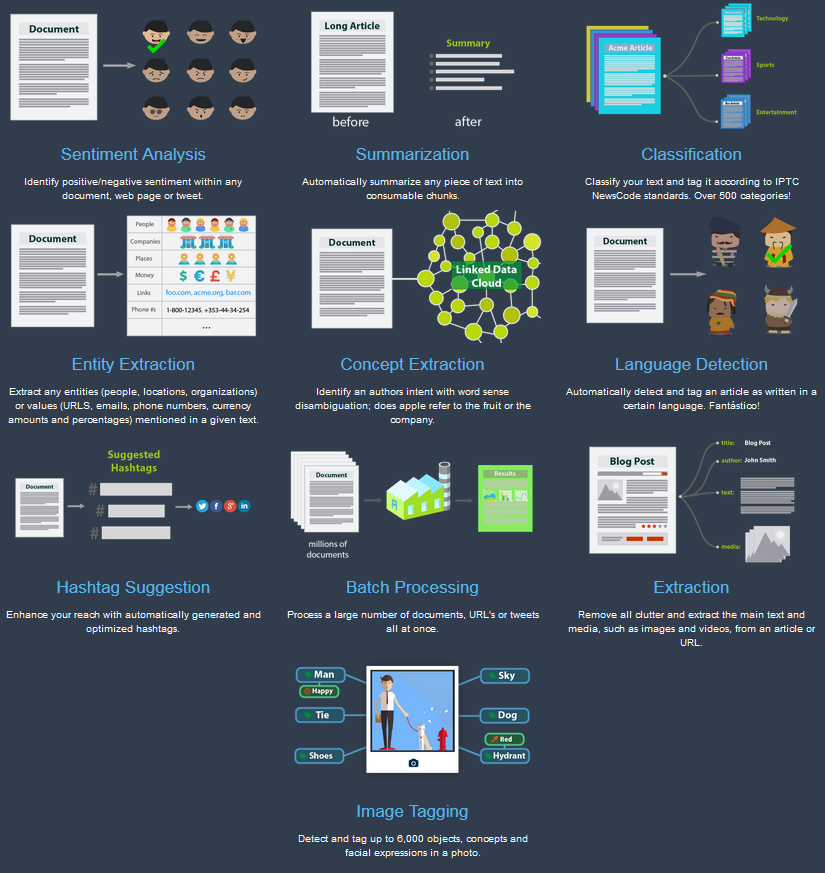
\includegraphics[width=0.6\linewidth,keepaspectratio]{nlp_overview}
\end{center}
\end{frame}
